\documentclass[11pt,a4paper]{article}

\usepackage[margin=2.5cm]{geometry}
\usepackage{amsmath,amssymb}
\usepackage{graphicx}
\usepackage{booktabs}
\usepackage{siunitx}
\usepackage{hyperref}
\usepackage{caption}
\usepackage{subcaption}
\usepackage{float}

\graphicspath{{../figures/}}

\hypersetup{colorlinks=true, linkcolor=blue, citecolor=blue, urlcolor=blue}

\title{Inferring Strong Gravitational Lens Parameters from Images\\
       with Simulation-Based Inference}
\author{Strong Lens Inference Project}
\date{July 2026}

\begin{document}

\maketitle

\begin{abstract}
We infer the physical parameters of strong gravitational lens systems directly from
single noisy images using amortized simulation-based inference (SBI). A forward model
built with \texttt{lenstronomy} simulates $64\times64$-pixel images of a singular
isothermal ellipsoid (SIE) lens with external shear magnifying a S\'ersic source,
including PSF convolution and realistic Gaussian and Poisson noise. A BayesFlow
neural posterior estimator---a convolutional summary network coupled to a conditional
normalizing flow---is trained on $8{,}000$ simulated image--parameter pairs and
evaluated on $300$ held-out systems. The Einstein radius, source position, and source
size are recovered accurately ($R^2 = 0.88$--$0.95$), the lens ellipticity moderately
($R^2 \approx 0.5$), while external shear remains largely unconstrained at the
signal-to-noise ratio of our images, consistent with physical expectations.
Simulation-based calibration reveals mild overconfidence of the learned posteriors for
the best-constrained parameters. Finally, extending the parameter vector with an
external convergence $\kappa$ reproduces the classical mass-sheet degeneracy: the
$\kappa$ posterior contracts only $12\%$ relative to the prior while exhibiting a
strong anti-correlation with the Einstein radius
($\langle\mathrm{corr}(\kappa,\theta_E)\rangle = -0.83$). Training the model takes
under twenty minutes on a consumer GPU (NVIDIA RTX~3060), after which posterior
sampling for a new lens image takes milliseconds.
\end{abstract}

\section{Introduction}

Strong gravitational lensing occurs when a massive foreground galaxy bends the light
of a distant background source, producing arcs, multiple images, or complete Einstein
rings. The observed image morphology encodes the projected mass distribution of the
lens: the ring radius traces the total enclosed mass (via the Einstein radius
$\theta_E$), the arc shapes trace the lens ellipticity, and subtle distortions trace
the tidal field of neighbouring structures (external shear). Extracting these
parameters from images is a core task in astrophysical applications ranging from
measuring dark-matter substructure to time-delay cosmography.

Classical lens modelling fits a parametric model to each image with
likelihood-based sampling (e.g.\ MCMC), which is accurate but slow---often hours per
system---and must be repeated from scratch for every new image. Upcoming surveys
(Euclid, LSST) are expected to discover $10^4$--$10^5$ new lenses, making per-system
MCMC impractical. \emph{Amortized} simulation-based inference offers an alternative:
a neural network is trained once on simulated (parameter, image) pairs to approximate
the posterior $p(\boldsymbol\theta \mid \mathbf{x})$, after which inference for any
new image requires only a forward pass. We implement this approach with
BayesFlow~\cite{radev2020bayesflow,bayesflow2023software}, using
\texttt{lenstronomy}~\cite{birrer2018lenstronomy} as the simulator.

Two questions structure the analysis:
\begin{enumerate}
    \item How well can each lens and source parameter be recovered from a single
          noisy image, and are the inferred uncertainties statistically calibrated?
    \item When an external convergence $\kappa$ (a uniform mass sheet) is added to
          the model, does the inference correctly reflect the well-known
          \emph{mass-sheet degeneracy}---i.e.\ report that $\kappa$ is essentially
          unidentifiable from a single image rather than hallucinating a tight
          constraint?
\end{enumerate}

\section{Forward Model and Simulated Data}

\subsection{Lens and source model}

Each system consists of a singular isothermal ellipsoid (SIE) lens with external
shear, magnifying a S\'ersic source. The inferred parameter vector is
\begin{equation}
\boldsymbol\theta =
(\theta_E,\; e_1,\; e_2,\; \gamma_1,\; \gamma_2,\; x_s,\; y_s,\; R_s)
\quad [\,+\;\kappa\,],
\end{equation}
where $\theta_E$ is the Einstein radius, $(e_1, e_2)$ the lens ellipticity
components, $(\gamma_1, \gamma_2)$ the external shear components, $(x_s, y_s)$ the
source position, $R_s$ the source half-light radius, and $\kappa$ the optional
external convergence (Section~\ref{sec:msd}). Following the assignment specification,
nuisance quantities are fixed and assumed known: the lens centroid (measurable from
the lens light), the source amplitude, the source S\'ersic index ($n=2$), and the
source-light ellipticity.

\subsection{Priors}

Parameters are drawn from independent uniform priors
(Table~\ref{tab:priors}). Ellipticity is sampled in axis ratio $q$ and position angle
$\phi$ and converted to $(e_1, e_2)$; shear is sampled in modulus $\gamma_{\rm ext}$
and angle $\phi_{\rm ext}$ and converted to $(\gamma_1, \gamma_2)$. Identical priors
are used at train and test time, a prerequisite for the calibration test in
Section~\ref{sec:calibration} to be valid.

\begin{table}[H]
\centering
\caption{Prior ranges. Lengths in arcsec, angles in radians.}
\label{tab:priors}
\begin{tabular}{lll}
\toprule
Parameter & Range & Meaning \\
\midrule
$\theta_E$          & $(0.7,\ 1.6)$    & Einstein radius \\
$q$                 & $(0.6,\ 1.0)$    & lens axis ratio $\rightarrow (e_1, e_2)$ \\
$\phi$              & $(0,\ \pi)$      & lens position angle \\
$\gamma_{\rm ext}$  & $(0,\ 0.08)$     & external shear modulus $\rightarrow (\gamma_1, \gamma_2)$ \\
$\phi_{\rm ext}$    & $(0,\ \pi)$      & external shear angle \\
$x_s,\ y_s$         & $(-0.3,\ 0.3)$   & source position \\
$R_s$               & $(0.05,\ 0.25)$  & source half-light radius \\
$\kappa$            & $(0,\ 0.20)$     & external convergence (only in the 9-parameter run) \\
\bottomrule
\end{tabular}
\end{table}

\subsection{Image simulation and noise}

Images are rendered on a $64\times64$ grid at $0.05''$/pixel (a $3.2''$ field of
view), convolved with a Gaussian PSF of FWHM $0.1''$, and degraded with Gaussian
background noise ($\sigma_{\rm bkg}=0.1$ per pixel) plus Poisson shot noise for an
effective exposure time of $100$\,s, using \texttt{lenstronomy}'s noise utilities.
With the adopted source amplitude the realized peak signal-to-noise ratio of the
dataset has median $\approx 4$ (range $\approx 1$--$8$), somewhat below the nominal
$10$--$30$ target; the images are therefore on the noisy end of realistic, which
should be kept in mind when interpreting the recovery results
(Section~\ref{sec:discussion}).

We precompute $N_{\rm train}=8{,}000$ training, $N_{\rm val}=1{,}000$ validation, and
$N_{\rm test}=300$ held-out test systems. Simulation is CPU-bound and parallelized
over worker processes; generation of the full dataset takes a few minutes on a
modern desktop.

\section{Inference Method}

\subsection{Neural posterior estimation with BayesFlow}

We use BayesFlow's neural posterior estimation: an \emph{amortized} approximation
$q_\phi(\boldsymbol\theta \mid \mathbf{x})$ to the posterior is trained by maximizing
the log-density of true parameters under the model across simulated pairs
$(\boldsymbol\theta, \mathbf{x}) \sim p(\boldsymbol\theta)\,p(\mathbf{x} \mid
\boldsymbol\theta)$. Two networks are learned jointly:

\paragraph{Summary network.} A compact convolutional network compresses each
$64\times64\times1$ image into a $48$-dimensional learned summary vector: three
convolutional blocks (two $3\times3$ convolutions each with $32$, $64$, and $128$
filters, followed by max-pooling and batch normalization), global average pooling,
and two dense layers. BayesFlow's built-in summary networks target sets and time
series, so this custom CNN is supplied for image data.

\paragraph{Inference network.} A conditional coupling-flow normalizing flow (depth
$4$) maps a standard Gaussian base distribution to the posterior over
$\boldsymbol\theta$, conditioned on the image summary. After training, posterior
sampling for a new image is a single forward pass---no MCMC.

The target parameters are standardized (z-scored) before entering the flow, since
they span very different numeric scales ($\theta_E \sim 1$ vs.\ $\gamma_i \sim
10^{-2}$).

\subsection{Training}

The approximator is trained offline on the precomputed dataset for $40$ epochs with
batch size $32$ and learning rate $10^{-3}$ (Keras~3 with the PyTorch backend). On an
NVIDIA GeForce RTX~3060 the full training run completes in under $20$ minutes; the
same configuration required $\approx 1.4$ hours on CPU, a speedup of roughly
$4$--$5\times$ end to end. Figure~\ref{fig:loss} shows the loss (negative
log-posterior density): the validation loss drops steeply within the first three
epochs and plateaus near $4.5$--$5.5$ after epoch $\sim$$17$, while the training loss
continues to decrease towards $\sim$$0.1$---clear evidence of overfitting in the
later epochs. Early stopping around epoch $20$ would likely yield an equally good or
better model in half the time (Section~\ref{sec:discussion}).

\begin{figure}[H]
\centering
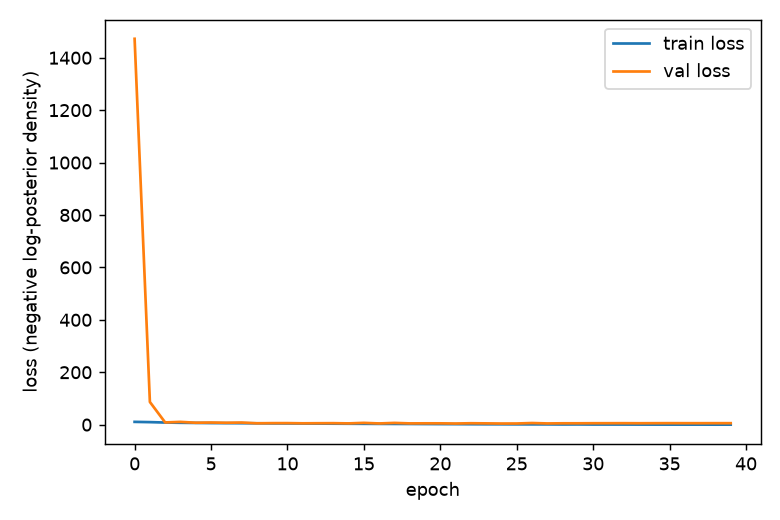
\includegraphics[width=0.62\textwidth]{training_loss.png}
\caption{Training and validation loss (negative log-posterior density). The
validation loss plateaus early while the training loss keeps decreasing, indicating
overfitting beyond roughly epoch 20.}
\label{fig:loss}
\end{figure}

\section{Results}

\subsection{Parameter recovery}
\label{sec:recovery}

Figure~\ref{fig:recovery} compares the posterior mean against the true value for each
parameter across the $300$ test systems ($2{,}000$ posterior samples per system);
Table~\ref{tab:r2} summarizes the coefficient of determination $R^2$.

\begin{table}[H]
\centering
\caption{Recovery accuracy (posterior mean vs.\ truth) on the 300-system test set.}
\label{tab:r2}
\begin{tabular}{lcl}
\toprule
Parameter & $R^2$ & Assessment \\
\midrule
$R_s$      & $0.95$ & excellent \\
$\theta_E$ & $0.88$ & very good \\
$y_s$      & $0.84$ & very good \\
$x_s$      & $0.83$ & very good \\
$e_2$      & $0.49$ & moderate \\
$e_1$      & $0.47$ & moderate \\
$\gamma_1$ & $0.21$ & poor \\
$\gamma_2$ & $0.06$ & essentially unconstrained \\
\bottomrule
\end{tabular}
\end{table}

\begin{figure}[H]
\centering
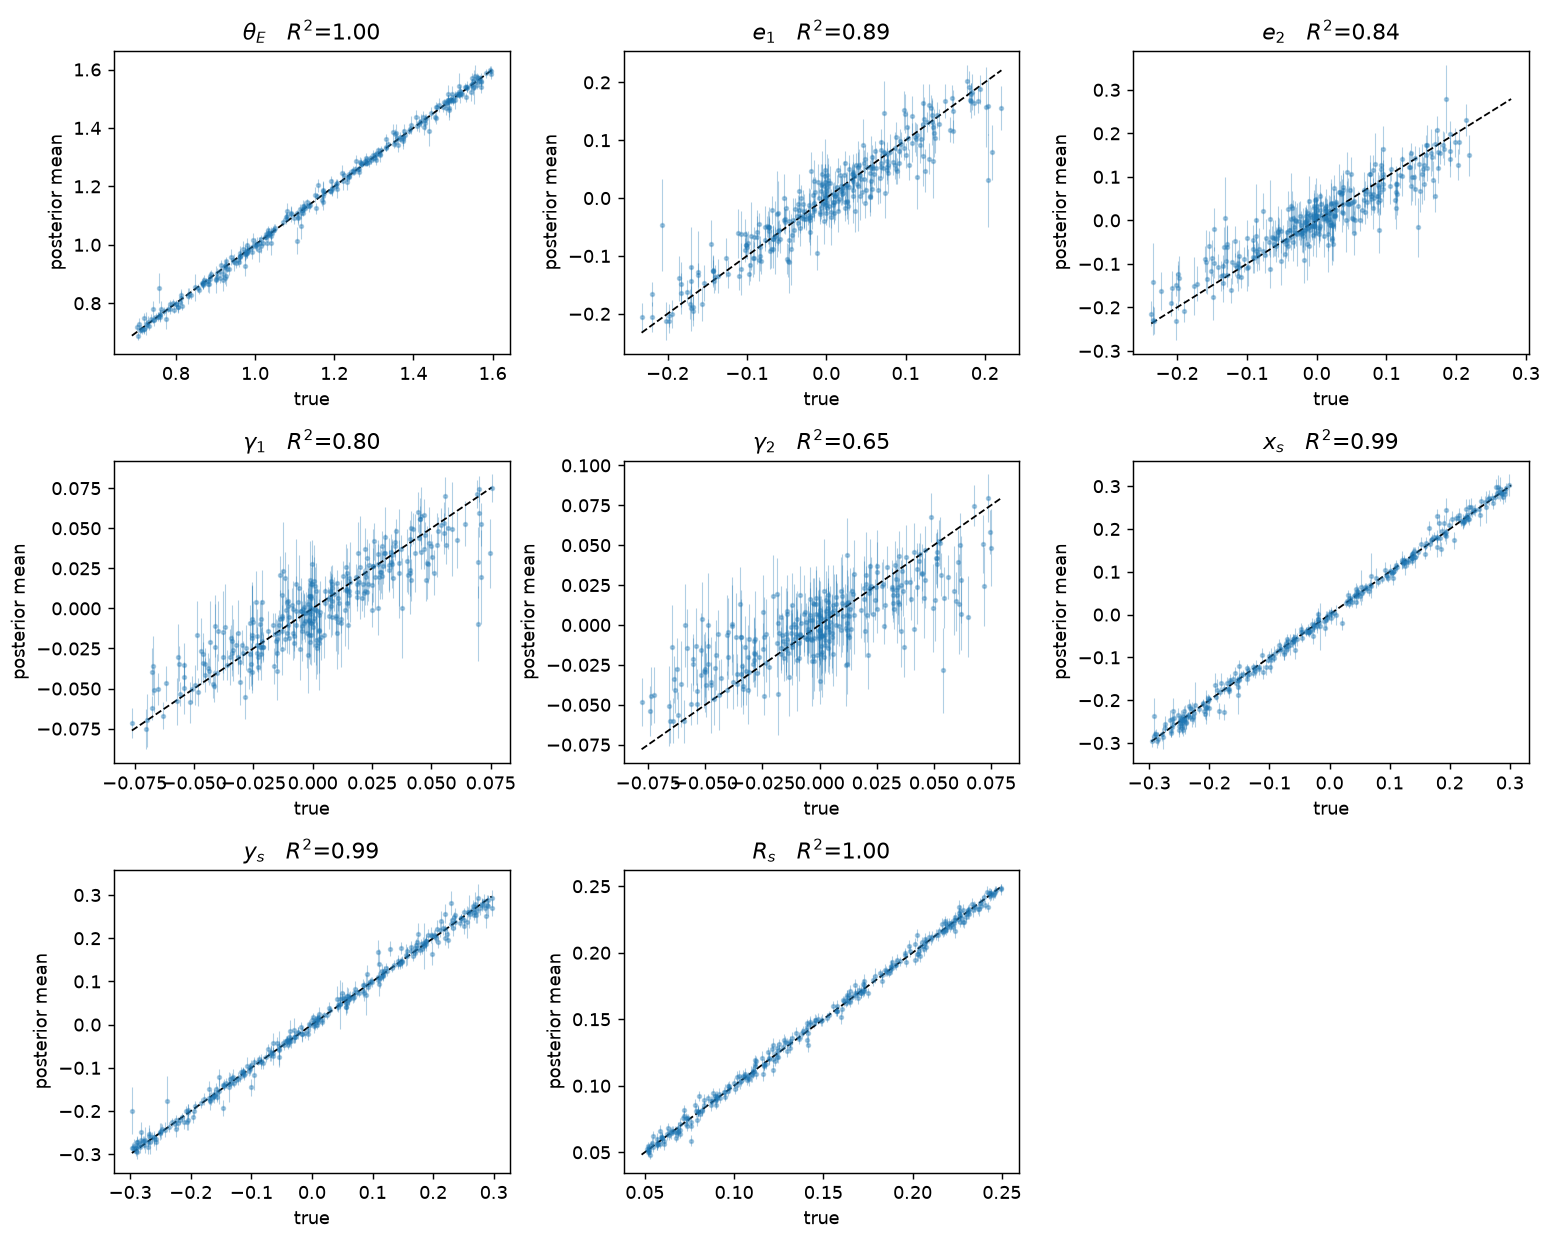
\includegraphics[width=\textwidth]{recovery.png}
\caption{Posterior mean vs.\ true value for each parameter over the held-out test
set. Error bars show the posterior standard deviation; the dashed line marks perfect
recovery.}
\label{fig:recovery}
\end{figure}

The hierarchy of recovery quality follows directly from how strongly each parameter
imprints on the image:

\begin{itemize}
    \item \textbf{Einstein radius, source position and size} ($\theta_E$, $x_s$,
    $y_s$, $R_s$): these set the ring radius, the arc configuration, and the arc
    thickness---large, direct morphological signatures---and are recovered with
    $R^2 \geq 0.83$. $R_s$ is the best-recovered parameter ($R^2=0.95$).
    \item \textbf{Lens ellipticity} ($e_1$, $e_2$): moderate recovery ($R^2 \approx
    0.5$) with visible shrinkage of extreme true values toward zero. This
    regression-to-the-prior-mean behaviour is expected for weakly identified
    parameters: where the likelihood is uninformative the posterior mean reverts
    toward the prior centre.
    \item \textbf{External shear} ($\gamma_1$, $\gamma_2$): poorly constrained
    ($R^2 = 0.21$ and $0.06$). This is physically reasonable rather than a network
    failure. The prior restricts the shear modulus to $\leq 0.08$, whose subtle
    quadrupole distortion of the arcs is comparable to, and partially degenerate
    with, the effect of lens ellipticity---and it is easily buried at the
    median peak SNR of $\sim$$4$ of these images. The wide error bars in
    Figure~\ref{fig:recovery} show the posterior itself ``knows'' shear is
    uncertain, which is exactly the desired behaviour of a well-behaved posterior
    (contrast with the calibration caveats below).
\end{itemize}

\subsection{Calibration (simulation-based calibration)}
\label{sec:calibration}

Accuracy of the posterior mean is not sufficient; the posterior \emph{width} must
also be statistically correct. We use simulation-based calibration
(SBC)~\cite{talts2018sbc}: for each test system the rank of the true parameter within
the posterior samples is computed; if the posterior is calibrated, ranks are uniform,
so the histograms in Figure~\ref{fig:calibration} should be flat within the grey
$99\%$ band.

\begin{figure}[H]
\centering
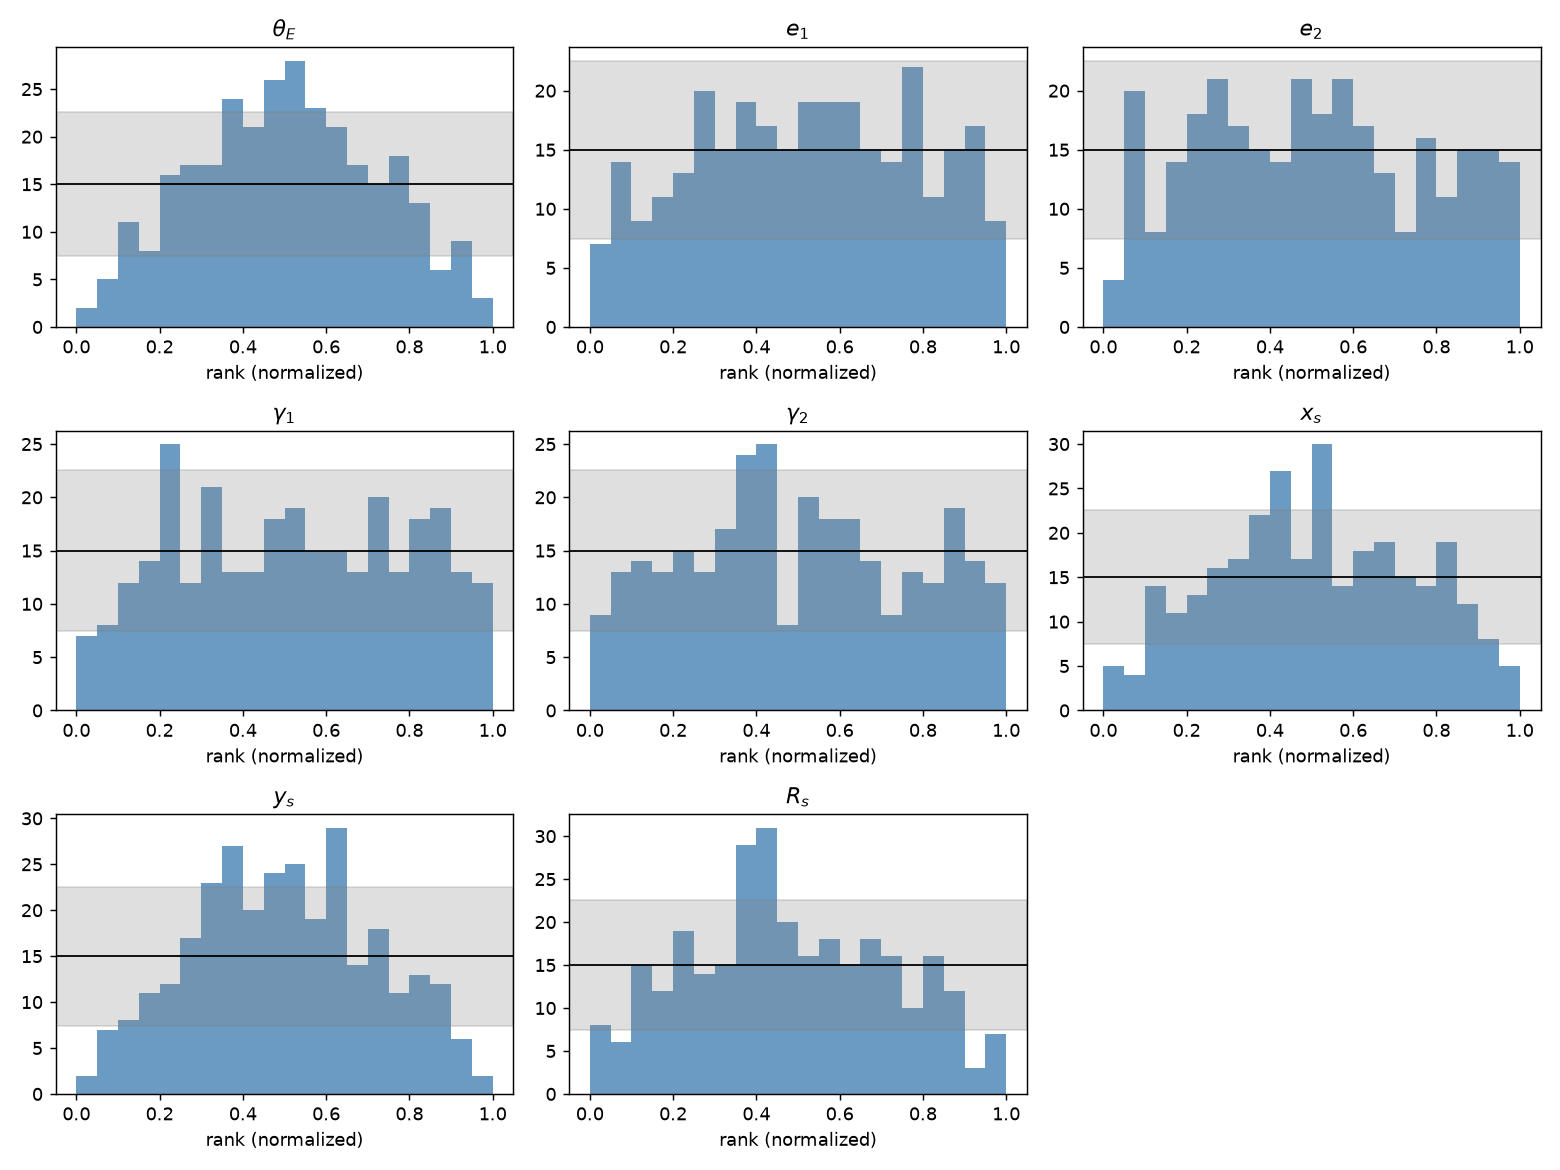
\includegraphics[width=\textwidth]{calibration.png}
\caption{SBC rank histograms per parameter. Flat within the grey band indicates a
calibrated posterior; a U-shape indicates overconfidence (posteriors too narrow).}
\label{fig:calibration}
\end{figure}

The histograms reveal a consistent pattern:

\begin{itemize}
    \item $\gamma_1$ and, to a lesser degree, $e_2$ are close to flat---the
    parameters the network constrains weakly inherit their width mostly from the
    prior, which is trivially calibrated.
    \item The well-recovered parameters ($x_s$, $y_s$, $R_s$, $\theta_E$) show clear
    U-shapes with mass piled at ranks $0$ and $1$: the true value falls in the
    extreme tails of the posterior more often than it should. The learned posteriors
    for these parameters are therefore \emph{overconfident}---too narrow by a
    modest factor.
\end{itemize}

This overconfidence is a common failure mode of neural posterior estimators trained
to convergence on limited data, and it is consistent with the overfitting seen in
Figure~\ref{fig:loss}: as the network memorizes training noise it becomes
increasingly (and unjustifiably) certain. Practical mitigations are discussed in
Section~\ref{sec:discussion}. The practical implication is that credible intervals
for the well-constrained parameters should be inflated somewhat before being used
for downstream science.

\subsection{Posterior predictive check}

As a complementary end-to-end test, we re-simulate images from posterior draws and
compare them with the observed image (Figure~\ref{fig:ppc}). The posterior draws
reproduce the observed arc configuration---ring radius, the positions of the three
bright knots, and the overall azimuthal light distribution---demonstrating that the
posterior concentrates on parameter values that regenerate the data. Differences
between individual draws are small and concentrated in the brightness of the knots,
visualizing the residual posterior uncertainty.

\begin{figure}[H]
\centering
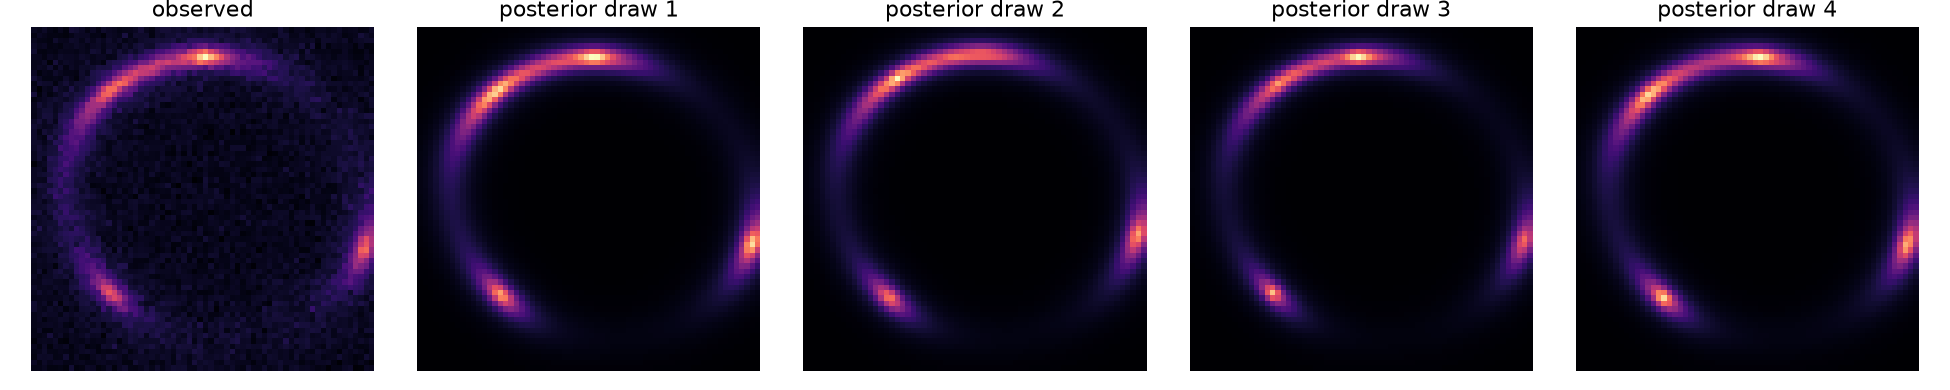
\includegraphics[width=\textwidth]{posterior_predictive.png}
\caption{Posterior predictive check for one test system: the observed noisy image
(left) and four noise-free re-simulations from independent posterior draws.}
\label{fig:ppc}
\end{figure}

\subsection{External convergence and the mass-sheet degeneracy}
\label{sec:msd}

A uniform sheet of external convergence $\kappa$ rescales the lens equation in a way
that is almost perfectly absorbed by a rescaling of the (unobservable) source plane:
image \emph{morphology} alone cannot distinguish $(\kappa, \theta_E)$ from a suitably
transformed pair. This is the classical \emph{mass-sheet degeneracy}, and a sound
inference pipeline must report it rather than hide it.

We repeat the full pipeline (generate, train, evaluate) with $\kappa \sim
\mathcal{U}(0, 0.2)$ added as a ninth inferred parameter. The results show exactly
the expected signature:

\begin{itemize}
    \item \textbf{Minimal posterior contraction.} The prior standard deviation of
    $\kappa$ is $0.058$; the mean posterior standard deviation across test systems is
    $0.051$, a contraction of only $12\%$. A single image leaves $\kappa$ almost as
    uncertain as the prior---the network has correctly learned that this parameter
    is nearly unidentifiable.
    \item \textbf{Strong internal anti-correlation.} Within individual posteriors the
    mean correlation between $\kappa$ and $\theta_E$ is $-0.83$: the two parameters
    trade off against each other along the degeneracy direction, exactly as the
    lensing equations predict (a larger mass sheet requires a smaller intrinsic
    Einstein radius to produce the same ring).
\end{itemize}

That an off-the-shelf neural posterior estimator recovers this degeneracy
structure---without being told about it---is a meaningful validation of the SBI
approach: the network reports joint posterior \emph{geometry}, not just marginal
point estimates. In practice, breaking this degeneracy requires external information
(stellar kinematics of the lens, time delays, or statistical priors on the
line-of-sight environment), none of which is present in a single image.

\section{Discussion and Limitations}
\label{sec:discussion}

\paragraph{Image signal-to-noise.} The realized peak SNR (median $\approx 4$) fell
below the nominal $10$--$30$ target, making this a stress test at the noisy end of
realistic conditions. Raising the source amplitude or lowering the background RMS to
hit the target range would likely improve ellipticity recovery substantially and
shear recovery marginally; the mass-sheet degeneracy conclusions would be unchanged,
as they are information-theoretic rather than noise-driven.

\paragraph{Overfitting and calibration.} Training for the full $40$ epochs past the
validation plateau produced overconfident posteriors for the well-constrained
parameters. Three inexpensive remedies, in increasing order of effort: early stopping
on validation loss (epoch $\sim$$20$); enlarging the training set (the simulator is
cheap---$50{,}000$ simulations remain feasible, and now that training runs on GPU the
enlarged dataset would still train quickly); and light regularization (dropout in
the summary CNN or weight decay).

\paragraph{Model scope.} The forward model fixes several quantities (lens centroid,
source amplitude and profile shape, PSF) that would be uncertain for real
observations, and simulates only the lensed source (no lens-galaxy light). Extending
$\boldsymbol\theta$ with these nuisance parameters, or marginalizing over them in the
simulator, is straightforward within the same pipeline and is the natural next step
toward application to survey data.

\paragraph{Computational profile.} With GPU training ($<20$ min) the pipeline
bottleneck is now dataset simulation ($\sim$$5$--$10$ min, CPU-parallelized). Once
trained, the amortized posterior costs milliseconds per system---the property that
makes this approach attractive for the $10^4$--$10^5$ lens samples expected from
upcoming surveys.

\section{Conclusion}

We built and validated an end-to-end amortized SBI pipeline for strong-lens parameter
inference. From single noisy $64\times64$ images, the BayesFlow posterior estimator
recovers the Einstein radius, source position, and source size accurately
($R^2=0.83$--$0.95$), the lens ellipticity moderately, and correctly assigns wide
uncertainties to external shear, which is nearly unidentifiable at the simulated
noise level. Simulation-based calibration exposes mild overconfidence in the
best-constrained parameters, attributable to overfitting and addressable with early
stopping and more training data. When external convergence is included, the inferred
posteriors exhibit the mass-sheet degeneracy exactly as theory predicts: negligible
contraction of $\kappa$ relative to the prior and a strong $\kappa$--$\theta_E$
anti-correlation ($-0.83$). The complete pipeline---simulation, training, and
evaluation---runs in about half an hour on a single consumer GPU, after which
inference on new systems is effectively instantaneous.

\begin{thebibliography}{9}

\bibitem{radev2020bayesflow}
S.~T. Radev, U.~K. Mertens, A.~Voss, L.~Ardizzone, and U.~K\"othe,
``BayesFlow: Learning complex stochastic models with invertible neural networks,''
\emph{IEEE Transactions on Neural Networks and Learning Systems}, 33(4):1452--1466, 2020.

\bibitem{bayesflow2023software}
S.~T. Radev, M.~Schmitt, L.~Schumacher, et al.,
``BayesFlow: Amortized Bayesian workflows with neural networks,''
\emph{Journal of Open Source Software}, 8(89):5702, 2023.

\bibitem{birrer2018lenstronomy}
S.~Birrer and A.~Amara,
``lenstronomy: Multi-purpose gravitational lens modelling software package,''
\emph{Physics of the Dark Universe}, 22:189--201, 2018.

\bibitem{talts2018sbc}
S.~Talts, M.~Betancourt, D.~Simpson, A.~Vehtari, and A.~Gelman,
``Validating Bayesian inference algorithms with simulation-based calibration,''
\emph{arXiv:1804.06788}, 2018.

\bibitem{schneider2013msd}
P.~Schneider and D.~Sluse,
``Mass-sheet degeneracy, power-law models and external convergence: Impact on the
determination of the Hubble constant from gravitational lensing,''
\emph{Astronomy \& Astrophysics}, 559:A37, 2013.

\end{thebibliography}

\end{document}
